\documentclass[conference]{IEEEtran}
\usepackage[T1]{fontenc}
\usepackage{mathptmx}
\usepackage{microtype}
\usepackage{amsmath,amssymb,amsthm}
\usepackage{booktabs,multirow,array,tabularx}
\usepackage{algorithm}
\usepackage{algpseudocode}
\usepackage{tikz}
\usetikzlibrary{arrows.meta,positioning,fit,calc,shapes.geometric,backgrounds,patterns}
\usepackage{pgfplots}
\usepgfplotslibrary{groupplots}
\pgfplotsset{compat=1.18}
\usepackage{xcolor}
\usepackage{xspace}
\usepackage{balance}
\usepackage[hidelinks]{hyperref}
\definecolor{navy}{RGB}{24,62,105}
\definecolor{teal}{RGB}{15,125,120}
\definecolor{amber}{RGB}{195,125,20}
\definecolor{slate}{RGB}{82,96,112}
\definecolor{metricBlue}{RGB}{41,104,168}
\definecolor{metricTeal}{RGB}{25,139,133}
\definecolor{metricAmber}{RGB}{210,143,36}
\definecolor{metricRed}{RGB}{187,82,78}
\definecolor{paleBlue}{RGB}{234,242,250}
\definecolor{paleTeal}{RGB}{232,247,245}
\definecolor{paleAmber}{RGB}{253,246,231}
\definecolor{paleRed}{RGB}{252,237,237}
\newcommand{\lgr}{\textsc{LGR}\xspace}
\newcommand{\reason}[1]{\texttt{#1}}
\newcommand{\set}[1]{\left\{#1\right\}}
\newtheorem{proposition}{Proposition}
\tikzset{
  flow/.style={-Latex, line width=.8pt, draw=slate},
  data/.style={draw=navy, fill=paleBlue, rounded corners=2pt, align=center,
               minimum height=9mm, text width=24mm, font=\footnotesize},
  stage/.style={draw=teal!85!black, fill=paleTeal, rounded corners=3pt, align=center,
                minimum height=10mm, text width=25mm, font=\footnotesize},
  govern/.style={draw=amber!85!black, fill=paleAmber, rounded corners=3pt, align=center,
                 minimum height=10mm, text width=25mm, font=\footnotesize},
  output/.style={draw=navy!85!black, fill=white, rounded corners=3pt, align=center,
                 minimum height=10mm, text width=27mm, font=\footnotesize},
  ledger/.style={draw=slate, fill=paleRed, rounded corners=2pt, align=left,
                 minimum height=7mm, text width=34mm, font=\scriptsize}
}
\begin{document}
\flushbottom
\title{Lifecycle-Governed Retrieval for Action-Safe Enterprise Knowledge Graphs}
\author{\IEEEauthorblockN{Amith Reddy Ravuru}
\IEEEauthorblockA{\textit{Independent Researcher}\\
San Francisco Bay Area, California, USA}}
\maketitle

\begin{abstract}
In enterprise knowledge graph retrieval systems, relevant evidence is not necessarily valid for the action it is used to justify. A retrieved fact may be outdated, replaced by a newer record, or incompatible with the policy governing the decision. This paper formalizes lifecycle-governed retrieval (\lgr), a decision procedure that connects evidence retrieval to action authorization. It represents facts as assertion events carrying validity periods, versions, and source information. \lgr first checks whether evidence is eligible for the requested decision, then resolves conflicting claims using declared source authority and record time, and finally checks whether policy and workflow rules permit the action. Only registered actions can be admitted; missing required authorization or evidence, or an unresolved conflict in evidence required for the action, prevents admission. Under stated assumptions, we establish that admitted actions that change external state satisfy the required policy and workflow conditions and rely on eligible evidence concerning the intended action target. The procedure records supporting evidence and reasons for its decisions, allowing the same decision record to be reproduced from an unchanged graph and governance snapshot. We provide an executable reference implementation and EvoMem-Enterprise, a synthetic benchmark covering changing facts, policies, and workflows. Pilot evaluations and targeted tests examine both retrieval quality and compliance with the specified decision rules, exposing failures that aggregate retrieval scores alone can miss. The contribution is an explicit, testable integration of evidence eligibility, conflict resolution, and action authorization, rather than a new retrieval algorithm. The evaluation supports this bounded systems design; it does not establish production safety or effectiveness with a deployed language model.
\end{abstract}
\begin{IEEEkeywords}
knowledge graph systems, enterprise memory, temporal knowledge graphs, provenance, ontology evolution, policy governance, workflow constraints, retrieval-augmented generation
\end{IEEEkeywords}

\section{Introduction}
\label{sec:intro}
Retrieval-augmented generation (RAG) grounds language models in external evidence \cite{lewis2020rag}, and graph-centric retrieval extends that evidence to entities, relations, neighborhoods, and multi-hop structures \cite{graphrag,kg2rag,graphflow,gretriever}. This suits enterprise assistance, where a response may depend on a customer, a contract, an entitlement, a policy, and a running workflow. Yet relevance ranking leaves a systems question unanswered: \emph{may the retrieved evidence support the requested decision now?}

The distinction matters when an assistant proposes an action rather than summarizes. Consider three cases: a support assistant retrieves a superseded entitlement; a service agent applies a service-level agreement (SLA) tier from the wrong policy version; a refund assistant finds a policy-eligible refund whose workflow has not reached the state permitting it. A related real-world failure illustrates the consequences of policy-inconsistent assistance: in \emph{Moffatt v.\ Air Canada} the B.C. Civil Resolution Tribunal held an airline liable after its chatbot answered a refund question with conditions contradicting the applicable bereavement-fare policy \cite{aircanada}. Fluent grounding is insufficient: evidence must also be current, attributable, semantically compatible, conflict-resolved, and action-admissible.

Prior work provides graph-based retrieval and associative memory \cite{graphrag,kg2rag,hipporag}, temporal and event-centered representations \cite{graphiti,e2rag,tgrag,kgirag,knowevolve}, conflict and evidence-governance mechanisms \cite{tgragconflict,truthfulrag,ledgerrag}, and process-aware retrieval \cite{grag4pm,a2jrag}. These do not by themselves define one deterministic contract ordering lifecycle, provenance, conflict, policy, and workflow checks before evidence can authorize an action. The composition carries design content no component forces: values must be normalized before conflicts can be grouped, guards must stay outside eligibility so evidence cannot authorize itself, and decision evidence must be completed beyond the top-$k$ context before any guard runs.

\lgr treats each fact as a versioned, time-bounded assertion event rather than a static triple: each separates a validity interval from a record time and carries lifecycle state, ontology and policy versions, provenance, and supersession links. \lgr filters assertions before action evaluation, resolves conflicts after normalization, and applies a registered default-deny gate; blocked items carry reasons, admitted effectful actions carry table-derived witnesses.

The paper makes four bounded contributions:
\begin{enumerate}
\item A knowledge graph (KG) systems architecture composing lifecycle eligibility, conflict resolution, governance tables, and action admission into a replayable decision packet, realized as an executable operator.
\item A formal, closed-world action model with a default-deny registry, a proposition that any admitted effectful action is registered, target-bound, guarded, evidenced, and conflict-free under stated assumptions, and a determinism proposition for its decision record.
\item EvoMem-Enterprise, a generated enterprise benchmark spanning ontology evolution, policy versions, provenance, supersession, contradictions, and workflow state.
\item A three-layer evaluation methodology separating retrieval correctness, decision conformance, and model behavior, instantiated by a validation-only label checker, a conformance suite with adversarial counterexamples, decisive strata, and a frozen pilot.
\end{enumerate}

\emph{Scope of claims.} Every empirical result here is a controlled design-and-pilot evaluation: the frozen pilot uses one generated world, and the pre-specified extension uses ten test worlds from the same generator family; both assume the supplied tables are correct, use a deterministic proxy in place of a language model, and include targeted branch testing. The paper claims a falsifiable specification, an executable reference behavior, and benchmark-level feasibility evidence---neither production readiness nor superiority over the systems in Section~\ref{sec:related}; Section~\ref{sec:validity} structures the residual threats.


\begin{figure*}[t]
\centering
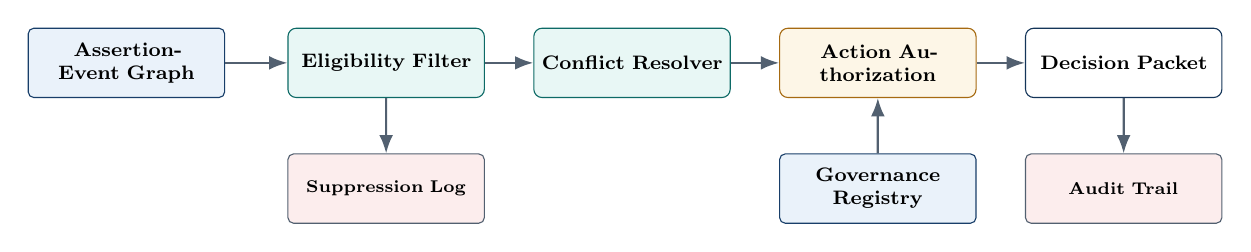
\begin{tikzpicture}[scale=.88, transform shape, node distance=8mm and 7mm]
  \node[data, text width=26mm, minimum height=10mm] (events) {\textbf{Assertion-Event Graph}};
  \node[stage, text width=26mm, minimum height=10mm, right=9mm of events] (eligibility) {\textbf{Eligibility Filter}};
  \node[stage, text width=26mm, minimum height=10mm, right=of eligibility] (conflict) {\textbf{Conflict Resolver}};
  \node[govern, text width=26mm, minimum height=10mm, right=of conflict] (authorization) {\textbf{Action Authorization}};
  \node[output, text width=26mm, minimum height=10mm, right=of authorization] (packet) {\textbf{Decision Packet}};
  \node[ledger, align=center, text width=26mm, minimum height=10mm, below=8mm of eligibility] (suppression) {\textbf{Suppression Log}};
  \node[data, text width=26mm, minimum height=10mm, below=8mm of authorization] (registry) {\textbf{Governance Registry}};
  \node[ledger, align=center, text width=26mm, minimum height=10mm, below=8mm of packet] (audit) {\textbf{Audit Trail}};
  \draw[flow] (events.east) -- (eligibility.west);
  \draw[flow] (eligibility.east) -- (conflict.west);
  \draw[flow] (conflict.east) -- (authorization.west);
  \draw[flow] (authorization.east) -- (packet.west);
  \draw[flow] (eligibility.south) -- (suppression.north);
  \draw[flow] (registry.north) -- (authorization.south);
  \draw[flow] (packet.south) -- (audit.north);
\end{tikzpicture}
\caption{\lgr architecture. Evidence flows left-to-right; the registry feeds authorization; filter and packet emit auditable outputs.}
\label{fig:architecture}
\end{figure*}

\section{Related Work and Novelty Boundary}
\label{sec:related}
GraphRAG, KG$^2$RAG, GraphFlow, and G-Retriever adapt the RAG pattern \cite{lewis2020rag} to graph topology, knowledge subgraphs, and graph-structured reasoning \cite{graphrag,kg2rag,graphflow,gretriever}, addressing candidate selection or answer synthesis. \lgr treats candidate generation as pluggable and imposes admission constraints afterward: relevance cannot compensate for an expired assertion, an incompatible mapping, or an unregistered action. HippoRAG is complementary associative-memory work, addressing how a generator retrieves long-term memory rather than whether that memory may support an action at decision time \cite{hipporag}.

The temporal core is deliberately standard and \lgr renames none of it: separating record time from validity interval is the transaction-time/valid-time distinction of bitemporal databases \cite{bitemporal}, standardized in SQL:2011 \cite{sql2011} and given semantic-web form by temporal RDF \cite{temporalrdf}; $\operatorname{TimeOK}$ is a textbook as-of predicate. Temporal KG research models time-varying events \cite{knowevolve}, and recent work brings entity-event graphs, time-sensitive retrieval, and document lineage to RAG and agent memory \cite{e2rag,tgrag,kgirag,graphiti,versionrag}. Against this lineage \lgr's delta is narrow: governance versions---ontology, policy, trust-table---participate in admission alongside bitemporal visibility, which none of these lines defines. Likewise its local closed-world decision rule adapts the local closed-world assumption of KB completion \cite{knowledgevault}; the asymmetric variant, in which unknown world facts stay unknown while unwitnessed authorizations become false, is this paper's framing.

Conflict-aware RAG studies disagreements between retrieved and parametric information or among changing sources \cite{tgragconflict,truthfulrag}; LedgerRAG keeps a claim-level ledger, adjudicates by authority and time, and can hold unresolved claims for review \cite{ledgerrag}; ordering conflicting defaults by priority while leaving incomparable residues undecided is prioritized defeasible reasoning \cite{defeasible}. \lgr claims no novelty for ledgers, authority-first adjudication, or the resolution logic: its resolver is a table-driven instance of prioritized defaults whose distinguishing behavior is that tied maxima stay unresolved and the gate treats that residue as blocking, per decision variable.

Process-aware retrieval has been explored for process mining and legal-information workflows \cite{grag4pm,a2jrag}, and runtime guardrails check agent actions against safety policies \cite{guardagent}. \lgr's workflow guard treats an externally modeled process such as BPMN \cite{bpmn} as a governance table consulted at admission time, not a retrieval target, and its gate differs from action-policy guardrails in what it consults: admission depends on the eligibility and conflict status of the supporting evidence, so a policy-permitted action is still blocked when that evidence is stale, unresolved, or unwitnessed. Remaining fields build on PROV-O \cite{prov}, RDF-star \cite{rdfstar}, SHACL \cite{shacl}, and XACML-style vocabularies \cite{xacml}; one baseline follows event sourcing \cite{eventsourcing}.

Overall, \lgr proposes no new retrieval, memory, temporal, conflict, or process method: its contribution is one compositional decision interface that knows which assertions were excluded and why, whether a conflict was resolved, which bindings authorize an action, and whether the decision reproduces from the same tables and graph state. It claims no learned retriever, no universal method for resolving truth, no organization-wide policy correctness, and no safe autonomous execution.

\section{System and Formal Model}
\label{sec:model}
\subsection{Assertion-event knowledge graph}
Let $G=(V,E,\mathit{type},\mathit{attr})$ be a typed graph with assertion-event nodes $A\subseteq V$; version, policy, workflow, source, and provenance nodes also lie in $V$. Each assertion event extends a subject--predicate--object statement with timestamps, versions, provenance, and lifecycle status:
\begin{equation}
a=\langle\tau,\sigma,\theta,\nu,\pi,\lambda,\psi\rangle,
\label{eq:assertion}
\end{equation}
where $\tau=(s,p,o)$ is the subject, predicate, and object; $\sigma=(\sigma_e,\sigma_r)$ the entity and relation scope; $\theta=(t_r,[v_f,v_u))$ the record time (transaction time: when the system learned it \cite{bitemporal}) and validity interval (valid time: when the fact held); $\nu=(\omega,\rho)$ the ontology and policy versions; $\pi=(\gamma,\mu)$ the provenance record and originating source; $\lambda\in\{\mathit{active},\mathit{superseded},\mathit{retracted}\}$ the lifecycle state; and $\psi$ an optional workflow binding. An implementation may also store the world-event time as metadata, as the released benchmark does; the predicates consume world time only through the validity interval, so the tuple omits it.

Supersession is a directed relation $R_{\mathrm{sup}}\subseteq A\times A$ rather than a tuple field, with $\operatorname{SupersededBy}(a)=\set{a'\in A:(a,a')\in R_{\mathrm{sup}}}$; an edge $(a,a')$ means $a'$ explicitly replaces $a$. A replacement takes effect once its record time is no later than $t_q$, and its later expiry or retraction does not revive $a$: a new value requires a new event. The implementation rejects dangling, cross-subject, and cyclic links.

Three notions meet in $\lambda$ and the model keeps them apart: assertion status, historical visibility, and removal policy. The \emph{superseded} status is induced by a visible replacement and carries its record time through $R_{\mathrm{sup}}$, so visibility follows from the log---a claim replaced on 1 June is visible as of 1 May and hidden as of 1 July, with no separate flag. \emph{Retraction} is a removal decision, such as a data-erasure obligation, and applies in every mode: a record retracted on 1 July is unavailable even as of 1 May. That asymmetry is why $\operatorname{LifeOK}$ is mode-scoped and why retraction carries no timestamp---a withdrawal is not a fact about when the claim held. Storage is unconstrained: metadata may attach to graph nodes, annotate RDF statements via RDF-star, or live in an event store.

A decision query is
\begin{equation}
q=\langle q_e,q_r,t_q,m_q,\beta_q,\omega_q,\rho_q,w_q,X_q,\mathcal{K}_q\rangle,
\label{eq:query}
\end{equation}
which separates entity/relation scope $q_e,q_r$, decision time $t_q$, query mode $m_q\in\set{\mathit{current},\mathit{historical}}$, an optionally declared action target $\beta_q$, target versions $\omega_q,\rho_q$, workflow instance/state $w_q$, candidate actions $X_q$, and the action-critical normalized keys $\mathcal{K}_q=\bigcup_{x\in X_q}\operatorname{Crit}(x)$ that those candidates require---so $\mathcal{K}_q$ is derived from the registry, not supplied independently, and $\operatorname{Crit}(x)$ of Section~\ref{sec:model}-C is its per-action component. Throughout, $T$ denotes the versioned governance bundle: the action registry, policy-family bindings and rules, workflow models and transitions, source catalog and relation-specific trust order, ontology mappings, provenance-activity registry, relation-semantics table, and snapshot metadata.

The underlying KG need not adopt global closed-world semantics. \lgr applies a \emph{local closed-world decision rule} to the snapshot available for $q$: absence of an assertion leaves a world fact unknown, but absence of a required registration, binding, or witness makes an effectful authorization false. That asymmetry is what default-deny needs---incomplete evidence may trigger abstention or escalation, never permission by open-world inference or a language model.

\begin{table}[t]
\caption{Decision-relevant assertion fields and their role.}
\label{tab:fields}
\centering\footnotesize\renewcommand{\arraystretch}{0.95}
\begin{tabular}{p{25mm}p{52mm}}
\toprule
\textbf{Field group} & \textbf{Decision role}\\
\midrule
Scope and time & Entity/relation coverage; record visibility; validity at $t_q$.\\
Lifecycle and lineage & Active/superseded/retracted status, explicit supersession, safe handling of stale records.\\
Versions & Mapping to $\omega_q$ and compatibility with the applicable $\rho_q$.\\
Provenance and trust & Registered activity, source class, and relation-specific authority order.\\
Conflict metadata & Query-normalized contradiction component; winner or unresolved outcome.\\
Governance bindings & Registry class, action target, policy rule, workflow transition, and guard witnesses.\\
\bottomrule
\end{tabular}
\end{table}

\subsection{Staged assertion eligibility and conflict resolution}
Trust is a versioned governance input. For policy version $\rho_q$, let
\begin{equation}
\operatorname{Trust}_{\rho_q}:(\hat p,\mu)\rightharpoonup\mathbb{Z}
\label{eq:trust}
\end{equation}
map a normalized relation and source to an authority tier. A governance owner builds it from a versioned source catalog and relation-specific precedence rules; the validator rejects duplicate assignments, missing tiers for declared action-relevant pairs, and a version inconsistent with $\rho_q$. Relations may use different orders, whose correctness remains an organizational assumption.

Normalization maps a predicate to at most one decision variable. The mapping table declares identity, rewrite, and split entries per ontology-version pair and distinguishes renaming classes from splits: several names may denote one variable across versions (\texttt{support\_plan}, \texttt{entitlement\_profile}, \texttt{support\_entitlement} here), each class having one canonical name, the name the trust and relation-semantics tables declare. $\operatorname{Norm}_{\omega_q}(p)$ collects the relations $p$ can reach, canonicalizes them, and returns the result if exactly one remains. If a split reaches two canonical names---distinct variables such as \texttt{support\_entitlement} and \texttt{product\_entitlement}---the mapping is \emph{ambiguous} and the assertion is ineligible (\reason{ontology-ambiguous}); resolving it by the order the query listed its relations would let syntax decide what a value means, so a value-transforming split must be declared as a rewrite per target relation. Canonicalization also stops a conflict hiding behind a rename: two records under different names normalize to one key and are compared.

$\kappa_q(a)$ denotes a normalized \emph{decision-variable} key such as $(\mathit{customer},\mathit{subscription\_status})$; the asserted object is deliberately not part of it. A versioned relation-semantics table declares whether distinct values are incompatible: single-value relations resolve, multi-value relations coexist. Since $\kappa_q$ is keyed by the canonical relation, every member of a conflict component shares one relation and the validator requires a trust order per canonical relation, so tiers are compared within one order, never across scales. Write $\kappa_q(Y)=\set{\kappa_q(a):a\in Y}$.

For a query $q$, a candidate assertion must satisfy eight predicates before it can be used by an action guard:
\begin{equation}
\begin{split}
\operatorname{Eligible}(a,q)\Leftrightarrow{}&
\operatorname{ScopeOK}\land\operatorname{TimeOK}\land\operatorname{LifeOK}\\
&\land\operatorname{OntOK}\land\operatorname{PolicyVerOK}\land\operatorname{ProvOK}\\
&\land\operatorname{SourceOK}\land\operatorname{SupOK}.
\end{split}
\label{eq:eligible}
\end{equation}
Eligibility is checked against the \emph{decision-evidence scope} $\hat q_r$---$q_r$ plus every relation the candidate actions' guards declare---not the retrieval scope $q_r$: otherwise the closure would gather a guard's witness and eligibility would discard it for not being a relation the query named, so narrowing a retrieval scope could silently change an authorization. Writing $t_r(a')$ for the record-time component of $a'$, and taking $\operatorname{Match}_{\omega_q}$ over $\hat q_r$, the predicates abbreviate the following checks against the versioned table bundle:
{\small
\begin{equation}
\begin{aligned}
\operatorname{ScopeOK}(a,q)&\Leftrightarrow
  \operatorname{Match}(\sigma_e,q_e)\land\operatorname{Match}_{\omega_q}(\sigma_r,\hat q_r),\\
\operatorname{TimeOK}(a,q)&\Leftrightarrow t_r\leq t_q\land t_q\in[v_f,v_u),\\
\operatorname{LifeOK}(a,q)&\Leftrightarrow \lambda=\mathit{active},\\
\operatorname{OntOK}(a,q)&\Leftrightarrow \omega=\omega_q
  \lor\operatorname{Map}_{\omega\rightarrow\omega_q}(p)\neq\bot,\\
\operatorname{PolicyVerOK}(a,q)&\Leftrightarrow
  \neg\operatorname{GovFact}(a)\ \lor\ \rho=\rho_q,\\
\operatorname{ProvOK}(a,q)&\Leftrightarrow
  \gamma\neq\bot\land\gamma\in\operatorname{dom}(\Gamma_T)\land\Gamma_T(\gamma)=\mu,\\
\operatorname{SourceOK}(a,q)&\Leftrightarrow
  \operatorname{Trust}_{\rho_q}(\hat p,\mu)\neq\bot,\\
\operatorname{SupOK}(a,q)&\Leftrightarrow
  \nexists a'\in \operatorname{SupersededBy}(a):t_r(a')\leq t_q.
\end{aligned}
\label{eq:predicates}
\end{equation}
}
$\operatorname{Match}(\sigma_e,q_e)$ holds when the assertion's subject or entity scope meets the query's, or its workflow instance is the query's; $\operatorname{Match}_{\omega_q}(\sigma_r,\hat q_r)$ when $\operatorname{Norm}_{\omega_q}(p)$ is defined and lies in the canonical image of $\hat q_r$; $\bot$ is an undefined mapping. $\Gamma_T$ is the declared provenance-activity registry carried in the governance bundle and held apart from the assertion stream, so a citation cannot vouch for itself. $\operatorname{ProvOK}$ fails on a citation that is absent from $\operatorname{dom}(\Gamma_T)$ or registered to another source. Because the condition is stated as membership in $\Gamma_T$ rather than as a lookup attempted only when $\Gamma_T$ is populated, an absent or empty registry resolves nothing and makes every citing assertion ineligible: a missing governance artifact withholds evidence rather than silently admitting it. The implementation additionally refuses to load a bundle whose registry file is missing or empty. A timestamp present but unparseable fails eligibility rather than reading as an open boundary. A visible successor permanently suppresses its predecessor while an unrecorded future one does not, and $\operatorname{GovFact}$ identifies policy and workflow assertions. Historical queries ($m_q=\mathit{historical}$) are evaluated at their audit time with $\operatorname{LifeOK}$ relaxed to $\lambda\neq\mathit{retracted}$, so superseded lineage stays explainable while a retracted record stays unavailable in every mode; by $\operatorname{ModeOK}$ they cannot authorize. The implementation records every failed predicate in a reason-coded suppression ledger. Crucially, neither a policy-action guard nor a workflow-action guard belongs to Eq.~\eqref{eq:eligible}: this avoids circular eligibility in which an action selects the evidence needed to authorize itself.

Candidate retrieval is not the evidence boundary. $\operatorname{Complete}(G,q,T)$ returns all snapshot assertions matching the query entity or workflow scope and any declared query, guard, conflict, or supersession dependency; it follows supersession links, records a completion manifest, and blocks rather than authorizes on a failed lookup. The first-stage set is
\begin{equation}
B_0(q)=\set{a\in\operatorname{Complete}(G,q,T):\operatorname{Eligible}(a,q)}.
\label{eq:bzero}
\end{equation}
For each single-value relation \lgr groups normalized assertions by $\kappa_q(a)$ and orders distinct values lexicographically by $\bigl(\operatorname{Trust}_{\rho_q}(\hat p,\mu),t_r\bigr)$, descending, retaining all top assertions supporting one winning value. $\operatorname{Losers}(q)$ is the eligible assertions supporting non-winning values of a uniquely resolved component, $\operatorname{Unresolved}(q)$ those in components whose incompatible maximum is tied. Multi-value relations bypass the resolver. A tied maximum is \emph{unresolved}: its members pass eligibility but are excluded from the decision-evidence set, so no member can witness an action:
\begin{equation}
B(q)=B_0(q)\setminus\bigl(\operatorname{Losers}(q)\cup\operatorname{Unresolved}(q)\bigr).
\label{eq:resolved}
\end{equation}
This is a reproducible protocol over an observed record, not a claim to determine truth; ranking orders members only after eligibility and conflict outcomes are fixed.

\smallskip
\noindent\textit{Worked decision sequence}, executable against the released tables. A customer has a \texttt{support\_entitlement=Premium} record from \texttt{crm} and a later \texttt{support\_entitlement=Standard} record from \texttt{billing}; the case state is recorded under the $\omega_1$ name \texttt{refund\_status=approved}, the subscription is \texttt{suspended}, and an $\omega_2$ \texttt{entitlement\_profile=Gold} record is also in scope. The query targets $\omega_3$. \texttt{refund\_status} reaches \texttt{workflow\_state} by a rewrite chain and canonicalizes to that one variable, so the case state is eligible under its current name. The \texttt{entitlement\_profile} record is not: its $\omega_2\!\rightarrow\!\omega_3$ mapping is a split reaching three distinct variables (\texttt{support\_entitlement}, \texttt{product\_entitlement}, \texttt{contractual\_entitlement}), and since normalization never consults the query, naming one of them cannot select a branch---the record is ineligible (\reason{ontology-ambiguous}). The two \texttt{support\_entitlement} records disagree, the relation is single-valued, and \texttt{billing} outranks \texttt{crm}, so the \texttt{crm} record is suppressed as a \reason{contradiction-loser}. The transition \texttt{approved}$\rightarrow$\texttt{refund\_issued} is enabled, but the refund rule also requires a non-suspended subscription, so \texttt{issue\_refund} is blocked \reason{guard-failed} with the enabled transition recorded beside the failure.

\subsection{Registered default-deny action admission}
\emph{Registry and bindings.} Let $X$ be the action identifiers and $\operatorname{Reg}:X\rightharpoonup\set{\mathit{advisory},\mathit{effectful}}$ the registry; an unregistered action is unavailable, not merely low-ranked. $\operatorname{Bind}_P$ and $\operatorname{Bind}_W$ map actions to versioned policy families and workflow models, and $\operatorname{Bound}(x,q)$ holds when every binding the query invokes is present and family-compatible, so a same-named rule from another family cannot authorize $x$. Write $\operatorname{Registered}(x)\Leftrightarrow x\in\mathrm{dom}(\operatorname{Reg})$, with $\operatorname{Advisory}$ and $\operatorname{Effectful}$ for the two classes.

\emph{Guards, witnesses, and the action target.} A \emph{guard atom} is one comparison in a policy rule or workflow transition, such as \texttt{workflow\_state} $=$ \texttt{approved}; its \emph{witness} is the eligible assertion whose value satisfies it. Eligibility alone does not make witnesses a justification, because eligible facts about different principals do not compose. An action is therefore evaluated against one \emph{action target} $\beta(q)=(\text{subject},\text{workflow instance})$, and only assertions bound to it may witness $x$: those whose subject or entity scope contains the target or whose workflow instance is the target's, plus governance facts, which are not entity-scoped.

$\beta(q)$ is resolved from declared relationships only. It is the query's declared target $\beta_q$ when one is given; otherwise, when $q$ names a workflow instance $w_q$, the target's members are the entities that $w_q$'s own workflow assertions declare as participants, intersected with $q_e$---and only assertions carrying $w_q$ from a source the trust table admits for \texttt{workflow\_state} may declare them, so no record can enrol an entity into a case it does not belong to. Membership is never inferred from the shape of an identifier: identifier spelling is a naming convention rather than an authorization relation, two unrelated entities may share any affix, and a case must keep its members when its identifier is renamed. When no declared relationship resolves the scope to one target, the action is refused (\reason{ambiguous-action-binding}) rather than evaluated against a mixture. $\operatorname{BindOK}(x,q)$ requires $\beta(q)$ to resolve to one target with every witness bound to it.

\emph{Conflict dependence and query mode.} Let $\operatorname{Crit}(x)$, declared in $x$'s registry entry, be the decision-variable keys whose unresolved status must block $x$; with $U$ the assertions in unresolved components, so $\kappa_q(U)$ is their key set, $\operatorname{CritOK}(x,q)\Leftrightarrow \operatorname{Crit}(x)\cap\kappa_q(U)=\emptyset$. The mode $m_q\in\set{\mathit{current},\mathit{historical}}$ is an explicit model input with $\operatorname{ModeOK}(x,q)\Leftrightarrow \operatorname{Advisory}(x)\lor m_q=\mathit{current}$: a historical query explains an earlier decision and never authorizes a new effectful one. Let $P(x,q,B)$ mean a family-compatible policy permit with no equal-or-higher-priority satisfied deny, and $W(x,q,B)$ an enabled workflow transition. Admission is then
{\small
\begin{gather}
\begin{aligned}
\operatorname{Admit}(x,q,B)\Leftrightarrow{}&
\operatorname{Registered}(x)\land\operatorname{ModeOK}(x,q)\\
&\land\operatorname{CritOK}(x,q)\land\operatorname{GovernedOK}(x,q,B),
\end{aligned}
\label{eq:admission}\\
\begin{aligned}
\operatorname{GovernedOK}(x,q,B)\Leftrightarrow{}&
\operatorname{Advisory}(x)\lor\bigl[\operatorname{Effectful}(x)\land\operatorname{Bound}(x,q)\\
&\land\operatorname{BindOK}(x,q)\land P(x,q,B)\land W(x,q,B)\bigr],
\end{aligned}
\label{eq:governed}
\end{gather}
}
An absent registration, binding, target, rule, transition, state, or witness makes an effectful action false. The output is an admitted action with its witnesses or a blocked one with a reason code (Fig.~\ref{fig:trace}), never a guessed authorization; each admitted action stores its witnesses with the rule and transition actually selected, so evaluation replays. The admitted set is $\operatorname{Adm}(q,B)=\set{x\in X_q:\operatorname{Admit}(x,q,B)}$.

The first proposition is a structural invariant of the definitions under its assumptions.
\begin{proposition}[Structural effectful-action soundness]
\label{prop:soundness}
Assume an immutable supplied snapshot whose declared dependencies are returned by $\operatorname{Complete}$, complete registry and binding tables for that snapshot, correct table-driven guard evaluation, a validated deterministic relation-semantics table, a deterministic conflict resolver that leaves tied maxima unresolved, and witnesses drawn only from $B(q)$. Each effectful $x\in \operatorname{Adm}(q,B(q))$ is registered, arises from a current-decision query, has a satisfied policy permit and workflow transition, has no equal-or-higher-priority satisfied deny, is supported by witnesses that satisfy Eq.~\eqref{eq:eligible} \emph{and are bound to one action target}, and depends on no unresolved critical conflict.
\end{proposition}
\begin{proof}
Equation~\eqref{eq:admission} excludes an unregistered action, a non-current query mode, and an unbound effectful action, and requires both satisfied guards. By Eqs.~\eqref{eq:bzero}--\eqref{eq:resolved}, guard witnesses are a subset of $B(q)$ and are therefore eligible, conflict winners, and not unresolved; $\operatorname{BindOK}$ additionally restricts them to assertions bound to the single target $\beta(q)$. The critical-key conjunct blocks any action depending on an unresolved component.\qedhere
\end{proof}
Proposition~\ref{prop:soundness} is definitional: it verifies that the contract cannot emit an effectful action lacking a required condition when operator and tables behave as assumed---not that an implementation is defect-free or that an organization's tables encode its policy. Its $\operatorname{BindOK}$ and $\operatorname{ModeOK}$ conjuncts are load-bearing: without the first, eligible facts about different principals compose into a justification no principal supports; without the second, an investigation query authorizes what it was meant to explain. Section~\ref{sec:audit} gives executable counterexamples for both.

Determinism, which the audit story rests on, is claimed for the \emph{decision record}---completed evidence identities, every suppression reason, the conflict outcome, and each action's verdict with its witnesses and selected rule and transition---not for a whole packet, which also carries the generator's retrieval context $R$ and runtime measurements such as latency.
\begin{proposition}[Determinism of the decision record]
\label{prop:replay}
Fix a snapshot $(G,T)$, a query $q$, and a feature configuration. Completion, predicate evaluation, normalization, the lexicographic resolver, and the table-driven gate are each pure functions of their inputs, with ties that no rule orders emitted as unresolved rather than broken arbitrarily. Two evaluations therefore yield an identical decision record, and hence an identical record digest, whatever candidate generator supplied $R$.
\end{proposition}
\begin{proof}
Each stage is a pure function of $(G,T,q)$, the configuration, and prior stages' outputs, and none consumes $R$: completion is defined over the snapshot and declared dependencies, not over the retrieval context. A composition of pure functions is pure, so the record is uniquely determined.\qedhere
\end{proof}


\begin{algorithm}[t]
\caption{Lifecycle-Governed Retrieval}
\label{alg:lgr}
\footnotesize
\begin{algorithmic}[1]
\Require graph $G$, query $q$ (with mode $m_q$), governance bundle $T$
\Ensure decision packet $\Pi$
\State $R\gets CandidateAssertions(G,q)$ \Comment{context, not the boundary}
\State $C\gets Complete(G,q,T)$; $B_0\gets\emptyset$; $L\gets\emptyset$
\State $Actions\gets\emptyset$; $Trace\gets\emptyset$
\State $D\gets SHA256(Canonicalize(G,T))$; $h\gets AssertionLogCheckpoint(G)$
\ForAll{$a\in C$}
  \State $r\gets FailureReasons(a,q,T)$ \Comment{Eqs.~\eqref{eq:eligible}--\eqref{eq:predicates}}
  \If{$r=\emptyset$} $B_0\gets B_0\cup\set{a}$ \Else $L\gets L\cup\set{(a,r)}$ \EndIf
\EndFor
\State $(B,U)\gets ResolveConflicts(B_0,\kappa_q,Trust_{\rho_q})$ \Comment{Eqs.~\eqref{eq:bzero}--\eqref{eq:resolved}}
\State $\beta\gets ActionTarget(q,B,T)$ \Comment{membership declared by $Trust$-eligible records only}
\ForAll{$x\in X_q$}
  \If{$\neg Registered(x)$ or $[Effectful(x)\land\neg Bound(x,q)]$} \Comment{registry}
    \State $Actions[x]\gets Block(x,\textit{unbound})$
  \ElsIf{$Effectful(x)\land m_q\neq\mathit{current}$} \Comment{Eq.~\eqref{eq:admission}: mode}
    \State $Actions[x]\gets Block(x,\textit{non-authorizing-query-mode})$
  \ElsIf{$Effectful(x)\land\neg Resolves(\beta)$} \Comment{one action target}
    \State $Actions[x]\gets Block(x,\textit{ambiguous-action-binding})$
  \ElsIf{$Crit(x)\cap\kappa_q(U)\neq\emptyset$} \Comment{critical conflict}
    \State $Actions[x]\gets Block(x,\textit{unresolved-conflict})$
  \ElsIf{$\neg GovernedOK(x,q,B)$} \Comment{Eq.~\eqref{eq:governed}}
    \State $Actions[x]\gets Block(x,\textit{guard-failed})$
  \Else
    \State $Actions[x]\gets Admitted(x,Witnesses_\beta(x,q,B,T))$ \Comment{witnesses bound to $\beta$}
  \EndIf
  \State $Trace\gets Trace\cup\set{(x,Actions[x],Rule(x),Transition(x))}$
\EndFor
\State \Return $\Pi=(R,C,B,L,U,Actions,Trace,D,h)$ \Comment{$C$, $U$, digest explicit}
\end{algorithmic}
\end{algorithm}

\begin{figure*}[t]
\centering
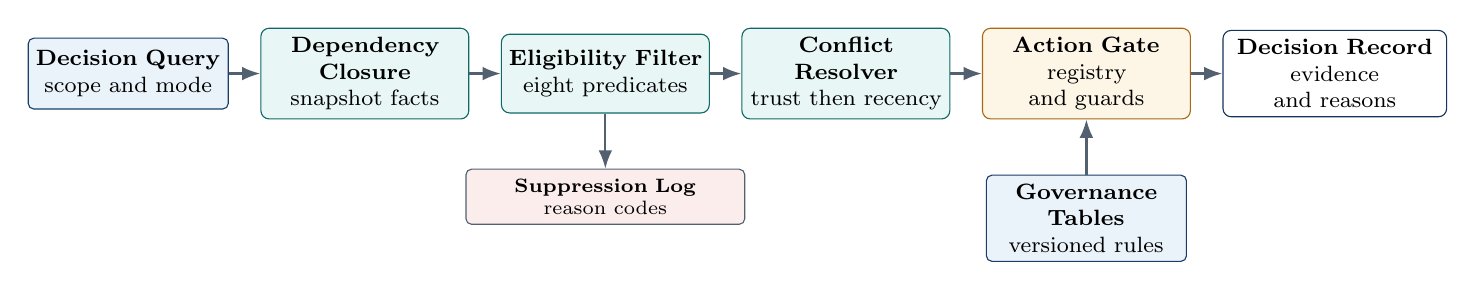
\begin{tikzpicture}[node distance=4mm, every node/.append style={text width=22mm, minimum height=13mm, inner xsep=2pt}]
  \node[data] (q) {\textbf{Decision Query}\\scope and mode};
  \node[stage, right=of q] (c) {\textbf{Dependency Closure}\\snapshot facts};
  \node[stage, right=of c] (b0) {\textbf{Eligibility Filter}\\eight predicates};
  \node[stage, right=of b0] (b) {\textbf{Conflict Resolver}\\trust then recency};
  \node[govern, right=of b] (g) {\textbf{Action Gate}\\registry and guards};
  \node[output, right=of g] (pk) {\textbf{Decision Record}\\evidence and reasons};
  \node[ledger, align=center, below=7mm of b0] (log) {\textbf{Suppression Log}\\reason codes};
  \node[data, below=7mm of g] (tables) {\textbf{Governance Tables}\\versioned rules};
  \draw[flow] (q) -- (c);
  \draw[flow] (c) -- (b0);
  \draw[flow] (b0) -- (b);
  \draw[flow] (b) -- (g);
  \draw[flow] (g) -- (pk);
  \draw[flow] (b0) -- (log);
  \draw[flow] (tables) -- (g);
\end{tikzpicture}
\caption{A query-level decision trace. Suppression reasons are recorded rather than hidden as implementation details.}
\label{fig:trace}
\end{figure*}

\subsection{Packet contract and evaluation layers}
Algorithm~\ref{alg:lgr} fixes the order, emitting $\Pi=(R,C,B,L,U,\mathit{Actions},\mathit{Trace},D,h)$, in which the completed set $C$, unresolved components $U$, suppression ledger $L$, digest $D$, and checkpoint $h$ are explicit outputs, not internal state. Figure~\ref{fig:architecture} gives the architecture, Fig.~\ref{fig:trace} one query-level trace, and Table~\ref{tab:fields} what each field decides. The storage layer maintains append-oriented assertion events with explicit relations to policies, ontologies, source activities, and workflow instances. A candidate generator---lexical, vector, graph-based, or hybrid---sits outside the safety boundary: it can improve the retrieval context but cannot emit an admissible action, because completion, eligibility, resolution, and the gate all run over the snapshot, not over its output.

The packet serializes accepted assertions with versions and provenance, excluded ones with reason codes, conflict components with winners and unresolved flags, action candidates with bindings consulted and guard witnesses, and a snapshot identifier: a SHA-256 digest over canonical ledger and table serializations plus the log checkpoint. A downstream large language model (LLM) may summarize or seek confirmation but must not treat absent evidence as approval; an implementation can require exact cited identifiers and reject outputs naming an action absent from the packet.

This separates three often conflated layers: \emph{retrieval correctness} (does the context a method returns carry the assertion events that $B(q)$ permits?), \emph{decision conformance} (does the evaluator implement Eqs.~\eqref{eq:eligible}--\eqref{eq:admission}?), and \emph{model behavior} (does an LLM use the packet correctly?). The original pilot and a pre-specified multiworld extension evaluate the first; targeted counterexamples and conformance tests evaluate selected branches of the second (Section~\ref{sec:audit}); no language model is run for the third.

\section{EvoMem-Enterprise Benchmark}
\label{sec:benchmark}
EvoMem-Enterprise stresses lifecycle and governance cases without exposing canonical timelines to retrieval. Following the reproducible-scenario spirit of temporal graph benchmarks \cite{tgb}, it models customer support, entitlement, SLA escalation, and refund decisions: each scenario has a canonical state timeline and produces an observed assertion-event stream with delayed recordings, stale facts, supersessions, ontology migration, policy changes, source-trust variation, contradictions, and workflow-state cases. Gold labels record eligible evidence, exclusions, conflict outcomes, packet support, and action expectations. Each assertion also carries a contradiction-group identifier as gold instrumentation only; the operator derives contradiction semantics from the versioned relation table and never reads it.

Table~\ref{tab:benchmark} summarizes the release; development and smoke tasks support debugging, not tuning. All frozen tasks share one world's entities, contradiction groups, and workflow instances; action metrics use only the 40 frozen action tasks, so one task moves an action match rate by 2.5 points. No temporal-QA or versioned-document benchmark can anchor this externally, because none carries the governance surface the operator consumes---versioned trust orders, policy families, transition tables, registry bindings \cite{tgb,versionrag}---and a hand-mapped slice would invent exactly the tables under test. An independently authored scenario set remains future work.

Action labels are derived from the canonical benchmark state and checked by a separately coded table interpreter that does not import the evaluated \lgr operator. All 60 action labels---40 frozen test, 15 development, and 5 smoke---agree with the versioned action registry, policy rules, and workflow tables: a consistency check within one generated world, not independent validation of the tables themselves.

\begin{table}[t]
\caption{EvoMem-Enterprise composition. Counts describe a generated benchmark, not an operational deployment.}
\label{tab:benchmark}
\centering\footnotesize\renewcommand{\arraystretch}{0.98}
\begin{tabularx}{\columnwidth}{@{}Xr@{}}
\toprule
\textbf{Artifact} & \textbf{Count}\\
\midrule
Entity-like nodes & 601\\
Assertion events / state changes & 611 / 215\\
Registered provenance activities & 600\\
Ontology versions / policy artifacts & 3 / 4\\
Workflow models / contradiction groups & 2 / 60\\
All evaluation tasks / frozen test tasks & 140 / 100\\
Action-labeled tasks (test / dev / smoke) & 40 / 15 / 5\\
Frozen tasks by label regime (satisfiable / retro. / out-of-scope) & 75 / 22 / 3\\
\bottomrule
\end{tabularx}
\end{table}

For the multiworld extension, a master seed is deterministically split into separate entity, event, contradiction, task, and split streams using SHA-256. Three development worlds support implementation checks, two validation worlds select the primary local comparator, and ten previously unevaluated test worlds provide the reported robustness result. A destination cannot be overwritten without an explicit force flag, every generated world is retained, and each world must pass structural, action-label, and evidence-label validation before evaluation. The version-3 labeling specification keeps retrospective and out-of-scope cases as diagnostic populations instead of deleting them; the primary population contains only current-decision tasks whose target is a minimal sufficient, contract-permitted evidence set. This changes the evaluation protocol, not the historical frozen release summarized in Table~\ref{tab:benchmark}.

\subsection{Methods and metric definitions}
\label{sec:metrics}
All frozen comparisons use $k=8$ retrieval-context items. The implemented generators are lexical top-$k$, recency-weighted retrieval, a 60-day time-to-live (TTL) filter, temporal-only KG retrieval, provenance-aware KG retrieval, ontology-versioned retrieval, a GraphRAG-style entity-seeded expansion, and an event-sourced latest-state proxy \cite{eventsourcing}; \lgr enables validity, lifecycle, provenance/trust, ontology/policy version, supersession, contradiction, and workflow features. These names identify released benchmark implementations, not reproductions of the systems in Section~\ref{sec:related}.

Let $R(u)$ be the retrieval context a method returns for task $u$ (at most $k$ identifiers) and $E(u)$, $S(u)$, $L(u)$ the gold eligible, stale-or-superseded, and contradiction-loser sets. Evidence metrics are computed on $R(u)$, not on the completed evidence, and macro-averaged. Eligible precision and recall are $|R\cap E|/|R|$ and $|R\cap E|/|E|$; F1 is their per-task harmonic mean. \emph{Stale non-exposure} is $|S\setminus R|/|S|$ and \emph{loser non-exposure} is $|L\setminus R|/|L|$ (each 1 when its gold set is empty): the per-task fraction of gold-flagged items kept out of the context. Both are reported beside eligible recall, since a method returning nothing attains 1.000 on each and only the pair separates withholding stale evidence from withholding all of it. Tasks are partitioned by label regime (Section~\ref{sec:results}): a task is \emph{satisfiable} when every assertion in $E(u)$ was recorded at or before the query instant, satisfies $\mathrm{ScopeOK}$, and survives conflict resolution, so that returning exactly $E(u)$ is permitted by the contract; \emph{retrospective} when some assertion in $E(u)$ was recorded later; and \emph{out-of-scope} when all were visible but some lies outside $\hat q_r$ or $q_e$. One script computes the time-and-scope partition; a separate validation-only interpreter independently checks eligibility and conflict survival without importing the evaluated operator or generator. Action-set agreement is the per-task indicator that the predicted valid-action set equals the gold set, over the 40 frozen action tasks. Context tokens are estimated as serialized-JSON length over four characters per token; latency is wall-clock retrieval-plus-admission time. The budget $k=8$ is fixed because no gold evidence set exceeds four assertions, so it never truncates a perfect selector. \lgr fills its context from its own completed, eligible, conflict-resolved set, ranked by requested-relation match, authority tier, and record time, appending witness identifiers the cutoff would drop; baselines fill theirs by their own scoring. Intervals are percentile intervals from 1{,}000 paired task-level bootstrap resamples.

The frozen-pilot intervals resample tasks. The multiworld primary interval instead uses 10{,}000 paired resamples of whole test worlds, preserving every method's observations within a sampled world.

For every main comparison the same completion and admission function follows the initial retrieval context, so a $k=8$ cutoff cannot change an action decision: action-set agreement is a conformance check for the common gate, not a measure on which generators can claim an advantage. A deterministic selector picks the first admitted action as a non-LLM execution proxy.

\section{Evaluation Results}
\label{sec:results}
\subsection{Frozen pilot}
The frozen split holds incompatible notions of a correct evidence set, so averaging them yields a target no behavior can maximize. A task's label is \emph{satisfiable} only when the admission contract permits an operator to return exactly its gold set: every gold-eligible assertion must be visible at the query instant, lie inside the query's declared entity and relation scope, and survive conflict resolution. Checking visibility alone is not enough, and the conditions fail for different reasons. A validation-only interpreter checks these requirements without importing the generator or evaluated operator. Of the 100 tasks, 75 are satisfiable, 22 are \emph{retrospective} (14 audit, 8 of 14 contradiction), requiring evidence recorded after the query instant, and 3 are visible in time but cite a relation outside the query's own scope, so the operator's scope rule forbids returning them. Table~\ref{tab:main} reports the first two apart and excludes the third, whose labels no scope-respecting operator can satisfy; the undifferentiated macro-average (0.722 for \lgr) obscures all three.

On the 75 satisfiable tasks \lgr attains eligible-assertion F1 of 0.963 (precision 0.949, recall 1.000) against 0.741 for provenance-aware KG retrieval, the strongest baseline: a paired bootstrap difference of $+0.222$, 95\% interval $[+0.193,+0.251]$ over 1{,}000 resamples. Its stale and contradiction-loser non-exposure are 1.000, exceeding the strongest baseline per metric by $+0.274$ $[+0.220,+0.333]$ and $+0.093$ $[+0.047,+0.147]$. Recall accompanies each non-exposure rate, since returning nothing also scores 1.000; perfect recall on this stratum shows \lgr withholds stale evidence, not all evidence.

On the 22 retrospective tasks \lgr scores 0.000 on F1 and recall, while baselines reach 0.32--0.51 by exposing records not yet visible. This favors neither: those labels ask for evidence the contract forbids at that instant, so the stratum measures label semantics, not retrieval quality, and no credit is claimed on it. The 3 out-of-scope tasks are a defect of the released labels rather than a regime: their gold sets cite relations the query never requested. Correcting both groups, or restating the retrospective ones against an audit-time target, is benchmark work this release does not do; the partition is reported so that neither is silently averaged into a headline.

Because the partition is derived from the same admission contract the operator implements, it is not an independent test of that contract, and the comparison on it is a post-hoc analysis of a split chosen after seeing the labels. Comparisons use whichever baseline is strongest per metric, with none excluded. Intervals stay descriptive: baselines were selected on this split, no multiplicity adjustment was applied, and tasks share entities and scenarios (Section~\ref{sec:validity}).

Every generator reaches exact action-set agreement of 1.000 on the 40 action tasks because the common gate, not its top-$k$ context, evaluates the action. One outlier is informative: ontology-versioned retrieval has the worst satisfiable-stratum stale non-exposure (0.393), below lexical top-$k$ (0.460), because its version-compatibility mapping widens matching to old-ontology names and surfaces disproportionately superseded assertions with no lineage check. Version-compatible retrieval is counterproductive on staleness unless composed with temporal and lineage checks. In the archived local run, \lgr uses 344.62 estimated tokens and 2.28\,ms mean latency, versus 380.27 and 1.68\,ms for the provenance-aware baseline; these support no efficiency conclusion.

\begin{table}[t]
\caption{Frozen-pilot evidence quality by label regime (Section~\ref{sec:metrics}). ``Satisfiable'' tasks are those whose gold evidence set the admission contract permits an operator to return; three further tasks are satisfiable in time but out of declared scope and are excluded from both columns. Stale and Loser are non-exposure rates, reported beside recall because returning nothing also scores 1.000. All methods share the completed gate, so action agreement is 1.000 for every method.}
\label{tab:main}
\centering\footnotesize\renewcommand{\arraystretch}{0.98}
\begin{tabular*}{\columnwidth}{@{\extracolsep{\fill}}lcccc|cc@{}}
\toprule
& \multicolumn{4}{c|}{\textbf{Satisfiable ($n{=}75$)}} & \multicolumn{2}{c}{\textbf{Retro. ($n{=}22$)}}\\
\textbf{Generator} & \textbf{F1} & \textbf{Rec.} & \textbf{Stale} & \textbf{Loser} & \textbf{F1} & \textbf{Rec.}\\
\midrule
Lexical top-$k$ & 0.392 & 1.000 & 0.460 & 0.747 & 0.335 & 1.000\\
Recency weighted & 0.687 & 0.993 & 0.687 & 0.753 & 0.477 & 0.773\\
TTL-only & 0.692 & 1.000 & 0.713 & 0.773 & 0.477 & 0.773\\
Temporal KG & 0.723 & 1.000 & 0.680 & 0.907 & 0.509 & 0.636\\
Provenance KG & 0.741 & 1.000 & 0.680 & 0.907 & 0.509 & 0.636\\
Ontology-versioned & 0.676 & 1.000 & 0.393 & 0.907 & 0.509 & 0.636\\
GraphRAG-style & 0.687 & 0.993 & 0.687 & 0.753 & 0.477 & 0.773\\
Event-sourced & 0.482 & 0.540 & 0.727 & 0.827 & 0.318 & 0.318\\
\textbf{\lgr} & \textbf{0.963} & 1.000 & \textbf{1.000} & \textbf{1.000} & 0.000 & 0.000\\
\bottomrule
\end{tabular*}
\end{table}

\subsection{Pre-specified multiworld evaluation}
The validation protocol selected provenance-aware KG retrieval as the strongest local comparator by mean eligible-evidence F1 across the two validation worlds. On the ten untouched test worlds, comprising 743 primary tasks, \lgr{} averages 0.961 F1 (world-level sample standard deviation 0.007), while the selected comparator averages 0.746 (standard deviation 0.009). The paired mean difference is $+0.215$, with a 95\% world-bootstrap interval of $[+0.212,+0.218]$. Every individual world difference is positive, ranging from $+0.206$ to $+0.224$ (Fig.~\ref{fig:multiworld}). \lgr{} has recall 1.000 and both stale and loser non-exposure 1.000 in every test world. These results establish consistency across seeds within one generator family; they do not establish transfer to independently authored scenarios or superiority over the published systems named in Section~\ref{sec:related}.

\begin{figure*}[t]
\centering
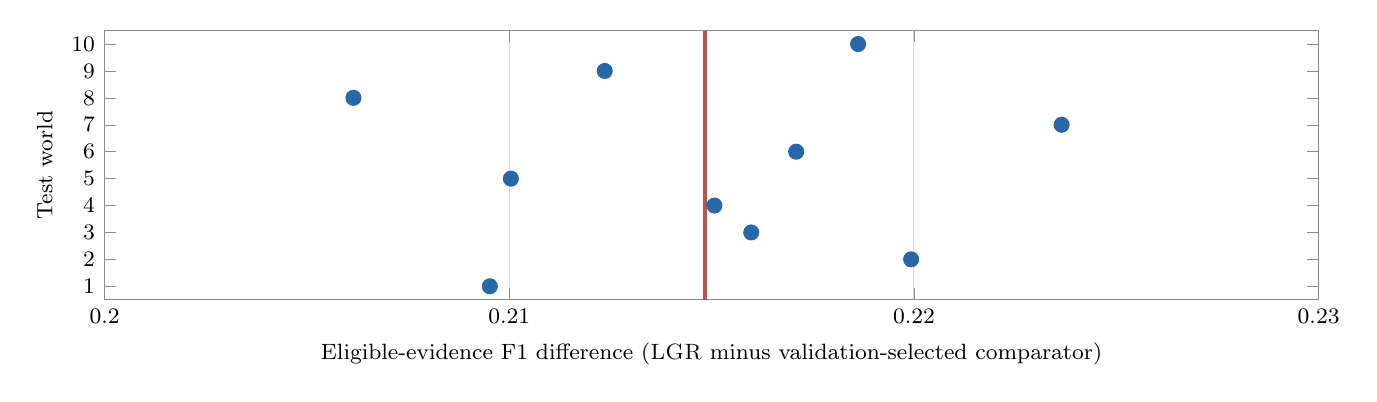
\begin{tikzpicture}
\begin{axis}[
  width=170mm,height=50mm,
  xmin=.20,xmax=.23,
  ymin=.5,ymax=10.5,
  xlabel={Eligible-evidence F1 difference (\textsc{LGR} minus validation-selected comparator)},
  ylabel={Test world},
  ytick={1,2,3,4,5,6,7,8,9,10},
  xtick={.20,.21,.22,.23},
  tick label style={font=\footnotesize},
  label style={font=\footnotesize},
  xmajorgrids=true,
  grid style={draw=black!15},
  axis line style={draw=black!45},tick style={draw=black!45}]
\addplot[only marks,mark=*,mark size=2.7pt,draw=metricBlue,fill=metricBlue] coordinates {
(.20952,1) (.21993,2) (.21598,3) (.21507,4) (.21004,5)
(.21709,6) (.22365,7) (.20615,8) (.21236,9) (.21862,10)};
\addplot[draw=metricRed,very thick,no marks] coordinates {(.21484,.5) (.21484,10.5)};
\end{axis}
\end{tikzpicture}
\caption{Paired F1 differences for all ten pre-specified test worlds. The vertical line marks the equal-weight mean ($+0.215$); no test world was excluded. Worlds differ by generated histories and task draws but share one generator family.}
\label{fig:multiworld}
\end{figure*}

A custom governance composition, written separately and importing neither the \lgr{} operator nor the generator, applies the same temporal, version, provenance, conflict, policy, workflow, and target-binding tables. Its admission path binds guard witnesses to one target and blocks actions that depend on an unresolved critical relation; separate two-account and unresolved-conflict regression cases exercise both safeguards. It reproduces \lgr's resolved evidence on all 1{,}500 tasks across development, validation, and test worlds and reproduces the table-derived action sets on all 635 action tasks. Equality is the informative result: the tested behavior can be assembled from conventional checks when their information, ordering, and fail-closed semantics are made identical. The empirical claim is therefore not that \lgr{} defeats every reasonable composition; its contribution is the explicit operator contract, trace, and conformance surface.

\subsection{Reference-implementation scaling}
Table~\ref{tab:scaling} measures the unindexed Python reference implementation on a 10-logical-CPU Apple-arm64 system using Python 3.9.6. Two stress modes separate total graph size from query-neighborhood size. In \emph{unrelated growth}, the completed dependency closure stays at 11 assertions while the snapshot grows; in \emph{dense growth}, nearly every added assertion enters the closure. Each cell summarizes 30 measured runs after five warm-ups for unrelated growth and three for dense growth. At 100{,}000 assertions, end-to-end p50 is 549\,ms with an 11-assertion closure and 2.98\,s with a 99{,}400-assertion closure. The result exposes the current implementation's full-snapshot scans and in-memory conflict grouping; it is not evidence of production-scale throughput. Snapshot digest time is reported separately because replay integrity has a cost even when the relevant neighborhood is small.

\begin{table}[t]
\caption{Reference-implementation scaling (milliseconds; 30 runs per row).}
\label{tab:scaling}
\centering\footnotesize\renewcommand{\arraystretch}{0.98}
\begin{tabular*}{\columnwidth}{@{\extracolsep{\fill}}lrrrrr@{}}
\toprule
\textbf{Growth} & \textbf{$|A|$} & \textbf{Closure} & \textbf{Digest} & \textbf{p50} & \textbf{p95}\\
\midrule
Unrelated & 1{,}000 & 11 & 5.61 & 1.46 & 2.11\\
Unrelated & 10{,}000 & 11 & 49.76 & 19.91 & 65.12\\
Unrelated & 100{,}000 & 11 & 513.59 & 548.58 & 594.57\\
Dense & 1{,}000 & 400 & 9.77 & 7.99 & 9.90\\
Dense & 10{,}000 & 9{,}400 & 47.94 & 194.24 & 268.54\\
Dense & 100{,}000 & 99{,}400 & 510.35 & 2{,}983.26 & 3{,}782.27\\
\bottomrule
\end{tabular*}
\end{table}

The ablation study now separates individual controls and reports two interactions explicitly (Fig.~\ref{fig:ablation}). Disabling relation-specific trust ranking lowers eligible F1 by 0.052, loser non-exposure by 0.080, and action-set agreement from 1.000 to 0.925; disabling conflict resolution lowers the same last two metrics and F1 by 0.027. Disabling workflow-instance scope lowers F1 by 0.058 but leaves action agreement unchanged. Action-target binding alone has no aggregate effect on this split, although the constructed two-account case in Section~\ref{sec:audit} shows that it decides an unsafe admission. Disabling record-time visibility alone lowers stale non-exposure by 0.140, while disabling valid time alone changes no aggregate metric because record visibility still excludes the retrospective evidence. Only the combined bitemporal ablation raises macro F1 by 0.033: retrospective F1 rises from 0.000 to 0.340, but its stale non-exposure falls from 1.000 to 0.364 and satisfiable-stratum F1 falls from 0.963 to 0.907. Similarly, the 15 action mismatches occur only when workflow-instance scope and action-target binding are disabled together; that combined ablation lowers action agreement to 0.625. These interaction results are not attributed to either control alone.

\begin{figure*}[t]
\centering
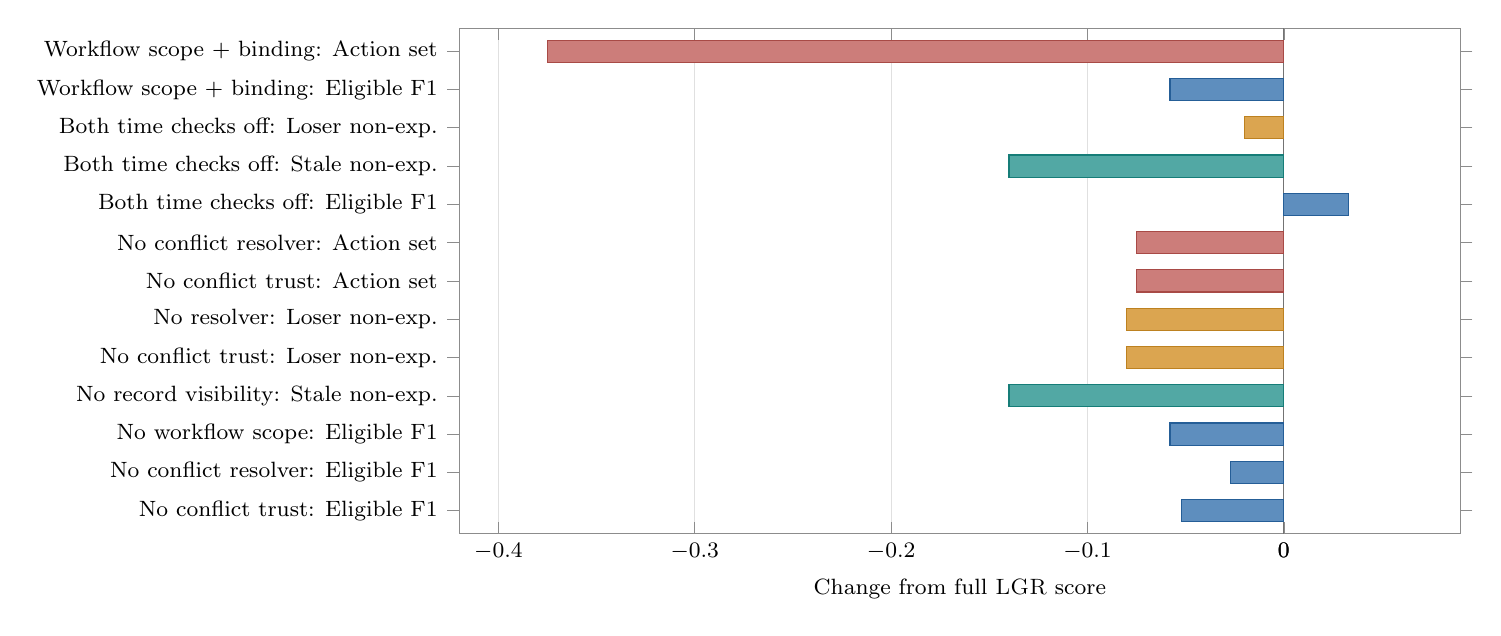
\begin{tikzpicture}
\begin{axis}[
  width=143mm, height=80mm,
  xbar, /pgf/bar width=8pt,
  xmin=-.42, xmax=.09,
  xlabel={Change from full \textsc{LGR} score},
  ytick={1,2,3,4,5,6,7,8,9,10,11,12,13},
  yticklabels={
    No conflict trust: Eligible F1,
    No conflict resolver: Eligible F1,
    No workflow scope: Eligible F1,
    No record visibility: Stale non-exp.,
    No conflict trust: Loser non-exp.,
    No resolver: Loser non-exp.,
    No conflict trust: Action set,
    No conflict resolver: Action set,
    Both time checks off: Eligible F1,
    Both time checks off: Stale non-exp.,
    Both time checks off: Loser non-exp.,
    Workflow scope + binding: Eligible F1,
    Workflow scope + binding: Action set},
  yticklabel style={font=\footnotesize, align=right},
  xtick={-.4,-.3,-.2,-.1,0},
  xticklabel style={font=\footnotesize},
  xlabel style={font=\footnotesize},
  xmajorgrids=true, ymajorgrids=false,
  grid style={draw=black!12},
  axis line style={draw=black!45}, tick style={draw=black!45},
  enlarge y limits=.05,
  extra x ticks={0}, extra x tick style={grid=major, grid style={draw=black!55}},
  clip=false]
\addplot[fill=metricBlue!75, draw=metricBlue!90!black, bar shift=0pt]
  coordinates {(-.052,1) (-.027,2) (-.058,3) (.033,9) (-.058,12)};
\addplot[fill=metricTeal!75, draw=metricTeal!90!black, bar shift=0pt] coordinates {(-.140,4) (-.140,10)};
\addplot[fill=metricAmber!80, draw=metricAmber!90!black, bar shift=0pt] coordinates {(-.080,5) (-.080,6) (-.020,11)};
\addplot[fill=metricRed!75, draw=metricRed!90!black, bar shift=0pt] coordinates {(-.075,7) (-.075,8) (-.375,13)};
\end{axis}
\end{tikzpicture}
\caption{Nonzero isolated-control changes and two explicitly combined interactions on the frozen pilot (ablated minus full \lgr, whole split). ``Both time checks'' means record-time visibility and valid time; the top two rows jointly remove workflow-instance scope and action-target binding. Every nonzero feature--metric change is plotted; the omitted pairs changed nothing to three decimals (Section~\ref{sec:decisive}).}
\label{fig:ablation}
\end{figure*}

\subsection{Zero-effect ablations, masking, and decisive strata}
\label{sec:decisive}
The lifecycle, ontology-version, policy-version, and supersession ablations change no aggregate metric, yet these are features the benchmark exists to stress. A released masking audit shows the null is structural, not sampling luck: every lifecycle-ineligible instance is also superseded and vice versa (118 of 118), every ontology-incompatible instance is already excluded by scope normalization and trust lookup (73 of 73; across all 61{,}100 task--assertion pairs a normalization failure implies a scope failure), and no wrong-policy-version fact survives other filters. An executable check confirms toggling any of the four flags changes eligibility membership nowhere. The release therefore adds ten decisive counterfactual tasks that one predicate alone decides: retraction without replacement (4), a replacement from a lower-authority source (3), and a wrong-regime policy fact with unclosed validity (3). On each, the full operator excludes the target for the intended sole reason and the ablation exposes it; twice the ablation admits an effectful refund the operator blocks. The zero deltas are a property of overlapping strata: redundancy the decisive strata show to be load-bearing.

The implementation also separates controls that the original broad flags coupled. Seven additional decisive cases isolate record visibility from valid time, provenance-activity resolution from source eligibility, workflow-instance scope from action-target binding, and source eligibility from relation-specific trust ranking. In each eligibility case the full configuration emits exactly the named reason and disabling only its flag removes that reason. The trust case changes the winner from an older higher-authority record to a newer lower-authority record; the target-binding case changes a blocked refund to an invalid admission supported by another account. These constructed cases demonstrate mechanism sensitivity, not prevalence or an aggregate effect size.

\begin{table*}[t]
\caption{Targeted conformance checks. ``Pass'' covers only the listed check.}
\label{tab:audit}
\centering\scriptsize\renewcommand{\arraystretch}{1.0}
\begin{tabularx}{\textwidth}{p{31mm}p{12mm}Xp{7mm}}
\toprule
\textbf{Requirement} & \textbf{Kind} & \textbf{Executable check} & \textbf{Result}\\
\midrule
Eligibility, normalization, conflicts, registry, guards, trust & Predicate & Negative cases for all eight predicates; future successor inert; invalid lineage, dangling and source-mismatched citations, and malformed instants rejected; cross-variable split rejected under either relation order; renamed relations normalize to one variable; equal-time incompatible maximum unresolved; advisory, unregistered, no-witness, cross-family and deny-precedence gating; duplicate trust tiers and version mismatch fail validation & Pass\\
Action target, scope, and mode & End-to-end & A second account in scope cannot witness the first's refund; unresolvable target refused; a guard witness survives a narrowed retrieval scope, leaving the admitted set unchanged; effectful actions blocked under a historical query & Pass\\
Decision record, replay, and decisive strata & End-to-end & Replays identically, excluding retrieval context and latency (Prop.~\ref{prop:replay}); rule and transition identities present; mutation changes the digest; sole-reason exclusion and ablated exposure on 10 original and 7 fine-grained control cases (Section~\ref{sec:decisive}), with effectful-action flips where applicable & Pass\\
Frozen-label verification & Label & Validation-only checkers derive action evidence from the assertion snapshot and test labeled evidence plus every duplicated stage-label view against eligibility and conflict resolution, importing neither operator nor generator; omissions, absent identifiers, malformed timestamps, and corrupted verdicts, witnesses, and reasons are detected; all 60 action labels and 75 permitted evidence labels pass & Pass\\
Generator conflict labels & Label & Independent generator fixtures cover authority before recency, recency within one tier, incompatible top ties, and equivalent top assertions; the two corrected historical owner cases remain regression fixtures & Pass\\
\bottomrule
\end{tabularx}
\end{table*}

\section{Executable Conformance Evaluation}
\label{sec:audit}
The implementation loads versioned action, trust, policy, workflow, ontology, provenance-activity, and conflict-semantics tables; completes declared dependencies; evaluates every action through one default-deny function; resolves query-normalized conflicts by relation-specific trust and descending record time (ties unresolved, no assertion-ID surrogate); and records the completion manifest, witnesses with their selected rule and transition, blocking reasons, digest, and checkpoint. Table~\ref{tab:audit} groups the operator suite's 34 cases over 29 declared requirement areas. Twenty-three further tests cover generator conflict semantics, validator mutations, and the standalone comparator, for 57 passing tests in total. Predicate cases exercise one control on a constructed world, end-to-end cases run the operator on benchmark tasks, and label checks compare frozen gold against independently derived reference evidence.

Thirteen of these cases are constructed counterexamples that the frozen split cannot exercise at all, because every action task carries one coherent case in scope, no audit task carries candidate actions, and no released mapping is ambiguous under a task's scope. Each pins an admission property on which the pilot's aggregate metrics are silent. The most consequential is cross-principal witnessing: with two accounts in scope---one suspended with an approved case, one active---nothing in the aggregate distinguishes a gate that refuses the first account's refund from one that authorizes it with the second account's subscription status. A related pair pins the \emph{basis} for that binding: because a case's participants are read from the membership its own workflow records declare, an unrelated account is excluded whether or not its identifier resembles the case's, and a case retains its members when its identifier is renamed. The rest cover an unresolvable action target, a guard dependency discarded by a narrowed retrieval scope, an effectful action admitted under a historical query, a split mapping resolved by relation or sort order, a renamed relation splitting one variable, dangling and unresolvable provenance, an empty or incomplete provenance registry, and malformed timestamps read as open boundaries. Every reported number is identical whether these properties hold or fail, which is the finding: a benchmark can be entirely silent about a soundness property that a single counterexample settles.

Label evidence is separated from generation: the generator writes labels back and cannot witness its own output, so the validation-only checkers import neither operator nor generator, write nothing, and fail on disagreement. The evidence checker independently derives contract-permitted candidates from the assertion snapshot, rejects malformed temporal fields, verifies every duplicated stage-label view, and detects a missing required answer witness. The action checker consumes that independently derived resolved set---not the supplied gold evidence---before re-deriving all 60 action verdicts, witnesses, and blocking reasons, including target binding and critical-conflict blocking. The evidence partition remains 75 permitted, 22 retrospective, and 3 out-of-scope test tasks with no failure in the permitted group. These checks still consume the same generated worlds and tables, so they establish consistency with those tables, not their organizational correctness.


\subsection{Scope of the conformance evidence}
Passing these cases is not implementation conformance: each is one branch on a constructed or benchmark input, establishing neither exhaustive verification nor the absence of a further counterexample of the kind Section~\ref{sec:audit} reports. The replay check detects changed local inputs but tests no durable store, concurrency, or log recovery; the label check verifies labels against the tables, not the tables against an organization.

The same-information custom composition and pre-specified ten-world evaluation close two earlier gates but also narrow the claim: conventional temporal, graph, and policy checks reproduce the tested operator when configured with the same tables and fail-closed order. Still open are independently authored scenarios and labels, alternative generator families and trust orders, a persistent indexed implementation under concurrent updates, durable recovery tests, and a fixed-version real-LLM evaluation reporting accuracy, invalid-admission rate, citation support, latency, tokens, and cost separately. SHACL or XACML \cite{shacl,xacml} are possible implementation substrates, but no claim of running either engine is made.

\section{Threats to Validity and Limitations}
\label{sec:validity}
\textit{Construct validity.} Exact action-set agreement measures whether the evaluator and a separately implemented interpreter reach the same result from the same closed-world tables---not that the tables are complete, that an LLM will follow the packet, or that an executed action is safe. Eligible F1 measures agreement with generated labels and is reported only within a declared regime. Non-exposure stays weaker than correct reason-coded suppression even when paired with recall. The composed comparator's exact agreement shows that the operator is implementable from its contract, but cannot validate a contract whose inputs both implementations share.

\textit{Internal validity.} The generator, tables, canonical evidence, composed comparator, and both label interpreters share scenario assumptions. Separate implementations reduce common-code errors but not common-specification errors. The masking audit quantifies how overlapping strata limit causal attribution, and the decisive strata and admission counterexamples restore it only in constructed worlds; untested properties may remain. The version-3 test seeds were fixed before their results were inspected, and every world was retained, but all were produced by one generator family.

\textit{Conclusion validity.} The original task-level bootstrap is post-hoc within one generated world and does not make its tasks independent. The extension selects one comparator on two validation worlds and resamples ten whole test worlds, so its interval measures seed variation within the generator more appropriately, but ten worlds remain a small engineering sample rather than a power-based design. No multiplicity adjustment is applied to secondary metrics, and the results do not cover alternative generator families, independently authored tables, or materially different trust orders.

\textit{External validity.} EvoMem-Enterprise is controlled and synthetic, representing neither naturally evolving corpora, extraction errors, organizational exceptions, adversarial data, nor local legal requirements. Multiple seeds improve robustness to generated variation, not to these omitted conditions. A protocol and blank template for independently authored scenarios are included, but no external contributor or real LLM evaluation is reported.

\textit{Limitations.}\label{sec:limitations} The formal results are conditional on a complete declared dependency closure, complete and correct registry, policy, workflow, ontology, provenance, trust, and relation-semantics tables, and a faithful implementation. They guarantee internal properties of the specified operator, not factual truth, legal compliance, fairness, privacy, or authorization beyond the modeled controls. The scaling harness uses synthetic replicas and an in-memory, unindexed Python implementation; its 100{,}000-assertion measurements neither predict a graph database nor exercise concurrent writes. The near-term use is decision support with explicit provenance and human confirmation for effectful operations; deployment must independently validate table ownership, update procedures, access controls, snapshot immutability, audit retention, recovery, and the packet--LLM interaction, none of which the local digest and replay tests discharge.

\section{Conclusion}
\lgr makes action admissibility a first-class KG systems problem: evidence must become eligible before it becomes persuasive, and an effectful action must become registered, targeted, and governed before it becomes available. On the 75 frozen-pilot tasks whose gold evidence the contract permits an operator to return, it reaches 0.963 eligible-evidence F1 against 0.741 for the strongest implemented local baseline at 1.000 recall with perfect stale and conflict-loser non-exposure. Across ten pre-specified test worlds and 743 primary tasks, the corresponding means are 0.961 and 0.746, a paired difference of $+0.215$ with a world-bootstrap interval of $[+0.212,+0.218]$. The claim is consistency under generated seed variation, not external validity.

The strongest lesson is that aggregate scores and conformance answer different questions. Admission properties such as cross-target witnesses, unresolved targets, historical query mode, split mappings, provenance resolution, and temporal integrity can remain invisible to a benchmark average; targeted counterexamples make those properties observable. Conversely, the same-information custom composition matches all tested \lgr{} evidence and action outputs, showing that no empirical advantage should be claimed over a faithfully composed implementation. The defensible contribution is a falsifiable contract, an executable trace, and evidence that its behavior is reproducible across the tested generated worlds. Independently authored scenarios, durable indexed replay, organizational policy review, and real-model evaluation remain necessary.

\section*{Data and Code Availability}
The submission artifact contains the frozen benchmark, the versioned labeling specification, all 15 multiworld datasets and per-task outputs, validation-only checkers, conformance and mutation tests, the standalone composed comparator, raw scaling timings, fixed protocols, and a no-mutation reproduction command. The archive is prepared as a release candidate and is released under the MIT license for both the code and the generated benchmark data; a public repository location and an archival identifier must still be assigned before the accepted version can claim public availability.

\section*{Acknowledgment}
The author used generative-AI tools for outline refinement and draft preparation, independently verified the final manuscript's claims, equations, results, and references, and assumes responsibility for its content.

\balance
\begin{thebibliography}{00}
\bibitem{lewis2020rag} P. Lewis \emph{et al.}, ``Retrieval-augmented generation for knowledge-intensive NLP tasks,'' in \emph{Proc. NeurIPS}, 2020.
\bibitem{graphrag} D. Edge \emph{et al.}, ``From local to global: A graph RAG approach to query-focused summarization,'' arXiv:2404.16130, 2024.
\bibitem{kg2rag} X. Zhu \emph{et al.}, ``Knowledge graph-guided retrieval augmented generation,'' in \emph{Proc. NAACL}, 2025.
\bibitem{graphflow} J. Yu \emph{et al.}, ``Can knowledge-graph-based RAG really retrieve what you need?'' in \emph{Proc. NeurIPS}, 2025.
\bibitem{gretriever} X. He \emph{et al.}, ``G-Retriever: Retrieval-augmented generation for textual graph understanding and question answering,'' in \emph{Proc. NeurIPS}, 2024.
\bibitem{aircanada} \emph{Moffatt v. Air Canada}, 2024 BCCRT 149, Feb. 2024.
\bibitem{hipporag} B. Jim\'enez Guti\'errez \emph{et al.}, ``HippoRAG: Neurobiologically inspired long-term memory for large language models,'' in \emph{Proc. NeurIPS}, 2024.
\bibitem{graphiti} P. Rasmussen \emph{et al.}, ``Zep: A temporal knowledge graph architecture for agent memory,'' arXiv:2501.13956, 2025.
\bibitem{e2rag} Z. Y. Zhang \emph{et al.}, ``Respecting temporal-causal consistency: Entity-event knowledge graph for retrieval-augmented generation,'' in \emph{Proc. EACL}, pp. 2017--2054, 2026.
\bibitem{tgrag} J. Han \emph{et al.}, ``RAG meets temporal graphs: Time-sensitive modeling and retrieval for evolving knowledge,'' arXiv:2510.13590, 2025.
\bibitem{kgirag} R. Yang \emph{et al.}, ``Beyond single pass, looping through time: KG-IRAG with iterative knowledge retrieval,'' arXiv:2503.14234, 2025.
\bibitem{knowevolve} R. Trivedi \emph{et al.}, ``Know-Evolve: Deep temporal reasoning for dynamic knowledge graphs,'' in \emph{Proc. ICML}, 2017.
\bibitem{tgragconflict} D. Li \emph{et al.}, ``T-GRAG: A dynamic GraphRAG framework for resolving temporal conflicts and redundancy in knowledge retrieval,'' in \emph{Proc. ACM Int. Conf. Multimedia (MM)}, 2025.
\bibitem{truthfulrag} S. Liu, Y.-M. Shang, and X. Zhang, ``TruthfulRAG: Resolving factual-level conflicts in retrieval-augmented generation with knowledge graphs,'' \emph{Proc. AAAI Conf. Artif. Intell.}, vol. 40, no. 38, pp. 32168--32176, 2026.
\bibitem{ledgerrag} S. Wang \emph{et al.}, ``LedgerRAG: Governance-driven agentic chain of retrieval for dynamic knowledge scenarios,'' \emph{Electronics}, vol. 15, no. 7, Art. 1376, 2026.
\bibitem{grag4pm} X. Su \emph{et al.}, ``GRAG4PM: Graph retrieval augmented generation framework adapted for process mining,'' \emph{Applied Sciences}, vol. 16, no. 10, Art. 5152, 2026.
\bibitem{a2jrag} T. Martin and S. Gilchrist, ``A2JRAG: Process-aware retrieval-augmented generation for public legal information systems,'' in \emph{AIDA2J Workshop, ICAIL}, 2026.
\bibitem{bitemporal} C. S. Jensen and R. T. Snodgrass, ``Temporal data management,'' \emph{IEEE TKDE}, vol. 11, no. 1, pp. 36--44, 1999.
\bibitem{sql2011} K. Kulkarni and J.-E. Michels, ``Temporal features in SQL:2011,'' \emph{SIGMOD Rec.}, vol. 41, no. 3, pp. 34--43, 2012.
\bibitem{temporalrdf} C. Gutierrez \emph{et al.}, ``Introducing time into RDF,'' \emph{IEEE TKDE}, vol. 19, no. 2, pp. 207--218, 2007.
\bibitem{versionrag} D. Huwiler, K. Stockinger, and J. F\"urst, ``VersionRAG: Version-aware retrieval-augmented generation for evolving documents,'' arXiv:2510.08109, 2025.
\bibitem{knowledgevault} X. Dong \emph{et al.}, ``Knowledge Vault: A web-scale approach to probabilistic knowledge fusion,'' in \emph{Proc. ACM SIGKDD}, 2014.
\bibitem{defeasible} G. Antoniou \emph{et al.}, ``Representation results for defeasible logic,'' \emph{ACM TOCL}, vol. 2, no. 2, pp. 255--287, 2001.
\bibitem{guardagent} Z. Xiang \emph{et al.}, ``GuardAgent: Safeguard LLM agents by a guard agent via knowledge-enabled reasoning,'' arXiv:2406.09187, 2024.
\bibitem{bpmn} Object Management Group, \emph{Business Process Model and Notation (BPMN), Version 2.0.2}, Dec. 2013.
\bibitem{prov} T. Lebo \emph{et al.}, Eds., \emph{PROV-O: The PROV Ontology}, W3C Recommendation, Apr. 2013.
\bibitem{rdfstar} O. Hartig \emph{et al.}, Eds., \emph{RDF-star and SPARQL-star}, W3C Community Group Final Report, Dec. 2021.
\bibitem{shacl} H. Knublauch and D. Kontokostas, Eds., \emph{Shapes Constraint Language (SHACL)}, W3C Recommendation, Jul. 2017.
\bibitem{xacml} OASIS, \emph{eXtensible Access Control Markup Language (XACML), Version 3.0}, Jan. 2013.
\bibitem{eventsourcing} M. Fowler, ``Event sourcing,'' martinfowler.com, 2005.
\bibitem{tgb} S. Huang \emph{et al.}, ``Temporal graph benchmark for machine learning on temporal graphs,'' in \emph{Proc. NeurIPS D\&B}, 2023.
\end{thebibliography}
\end{document}
